\chapter{Implementierung}%

\label{cha:Implementierung}
%was man alles anpassen muss
Es wurde sich für eine bestehende grundlegende Implementierung entschieden welche schon die Spiellogik von Vier Gewinnt sowie einen sehr einfachen reinforcement learning Ansatz enthält. In dieser Version lernt der Agent gegen einen Gegner zu gewinnen der zufällige Züge macht.\cite{connectfork}\\
Diese Implentierung wurde um einen Gegner erweitert der seine Züge nach dem Minimax Algorithmus auswählt.\\
Weitergehend wurde die reinforcement learning Implementierung überarbeitet um gegen den Minimax Algorithmus gewinnen zu können.\\
Diese Implementierungen werden hier einmal genauer beschrieben:\\

\subsection{Vier Gewinnt}
Die Implementierung des Spiels Vier Gewinnt deckt alle, für das Spiel wichtigen, Regeln ab. Es wird sich darum gekümmert welcher Spieler aktuell dran ist. Hat dieser sich dann für eine Action entschieden übernimmt das Spiel die korrekte Platzierung der Spielsteine, sowie die Überprüfung auf den Abschluss eines Spiels.\\ 
Es wurde sich dafür entschieden, dass der reinforcement learning Agent immer mit einer Partie beginnt, um somit die Menge an möglichen States zu halbieren, wodurch das gesammte Problem vereinfacht wird.

\section{Gegner mit Minimax Algorithmus}
Der Minimax Algorithmus wurde als Teil des Environments implementiert und besteht im Groben aus zwei Teilen. Einmal die Funktion $check\_next\_actions$ die den Suchbaum für die nächsten Züge aufbaut. Und die Funktion $find\_best\_move$ die den Suchbaum nach dem besten Zug durchsucht. Hierdurch kann sich dieser Gegner zu jedem State den besten nächsten Zug errechnen. Da dies im Optimalfall ein unschlagbarer Gegner ist wird hier noch mit einer Wahrscheinlichkeitsverteilung gearbeitet um den Gegner schlagbarer zu machen.

\subsection{check\_next\_actions}
Das Erstellen des Suchbaums funktioniert nach dem Negamax Algorithmus, es wird also eine Funktion für beide Spieler genutzt und immer abwechselnd das Maximum und das Minimum gesucht.

\subsection{find\_best\_move}
Das Suchen des besten Zuges wird durch die Alpha-Beta Suche beschleunigt indem bestimmte Äste des Suchbaumes, die sicher nicht zum gewünschten besten Zug führen, nicht weiter betrachtet werden. Dazu wurde noch eine Funktion zur Wahrscheinlichkeitsverteilung implementiert, die dafür sorgt, dass der Minimax Algorithmus in bestimmten Situationen mit einer gewissen Chance nicht optimal spielt.

\subsection{Wahrscheinlichkeitsverteilung}
Durch die Wahrscheinlichkeitsverteilung wird es ermöglicht einen zufälligen Zug aus den vom Minimax Algorithmus errechneten Zügen zu wählen. Hierbei macht die Gewinnchance eines Zuges aus, wie wahrscheinlich es ist, dass dieser ausgewählt wird. Diese Wahrscheinlichkeit kann mit einer $Variable$ angepasst werden, wodurch die  Wahrscheinlichkeit steigt dass einer der suboptimalen Züge, die vom Minimax Algorithmuses berechnet wurden, ausgewählt wird. 

\section{Gegner mit schlechten Strategien}
Um das Lernverhalten zu beobachten wurden zwei Gegner mit schlechten Strategien geschaffen.

\subsection{Gegner mit deterministischen Aktionen}
Es wurde ein Gegner geschaffen der zu jedem Zug immer so weit links wie möglich in das Spielfeld einwirft. 

\subsection{Gegner mit zufälligen Aktionen}
Es wurde ein Gegner geschaffen der zu jeden Zug in ein zufälliges Loch des Spielfeldes einwirft, das noch frei ist.


\section{Reinforcement Learning}
Für das reinforcement learning wird ein Deep Q-Network genutzt, welches einen Agenten an dem Environment trainiert. Im Folgenden wird die Implementierung der hierfür notwendigen Komponenten beschrieben. 


\subsection{Environment}
In Vier Gewinnt ist dies das Spielfeld und der Gegner. Das Spielfeld ist hier ein zweidimensionales Array der Länge 6 * 7. Der Gegner ist während des Lernens ein Computergegner der nach unterschiedlichen Strategien wie zum Beispiel dem Minimax Algorithmus handelt. \\

\subsection{Agent}
Der Agent ist einer der beiden Spieler von Vier Gewinnt, welcher lernt seine Züge durch die ihm gegebene Policy auszuwählen, um einen möglichst hohen Reward zu erhalten.\\

\subsection{State}
 Für Vier Gewinnt beschreibt der State welche der 42 Felder mit welchen Steinen befüllt sind. Ein Beispiel für so einen State kann man in dem Abschnitt \hyperref[sec:visualisierung]{Visualsierung des Spiels} finden.\\


\subsection{Actions}
Die Actions in Vier Gewinnt beschreiben die sieben Löcher in die der Agent Steine werfen kann.\\

\subsection{Reward}
 Zuerst wurde eine einfache diskrete Implementierung erstellt, welche den Reward immer zum Ende einer Partie ausgibt, wobei dieser beim Gewinn 1 beim Verlieren -1 und wenn die Partie unentschieden ausgeht 0 beträgt.
Dies wurde durch die Anzahl der Züge um eine kontinuierliche Komponente erweitert. Hierfür wird der Reward, der durch die diskrete Implementierung ermittelt wurde durch die Anzahl der Züge geteilt. Da es nicht möglich ist, vor dem vierten Zug zu gewinnen, wird erst ab diesem Zug gezählt. Es ergibt sich also die Formel: \\$$\frac{Reward}{Anzahl Züge-3}$$\\
Wie man in Abbildung \ref{fig:reward_function} gut sehen kann wird somit das schnelle Gewinnen mehr belohnt (obere Linie) und das schnelle Verlieren mehr bestraft (untere Linie). Da nur wenn das Spielfeld komplett voll ist unentschieden gespielt wird, wird hier ein Reward von 0 gegeben (einzelner Punkt). Diese Reward-Funktion wird im weiteren Text als zugabhängige Reward-Funktion benannt. \\

\begin{figure}[h!]
  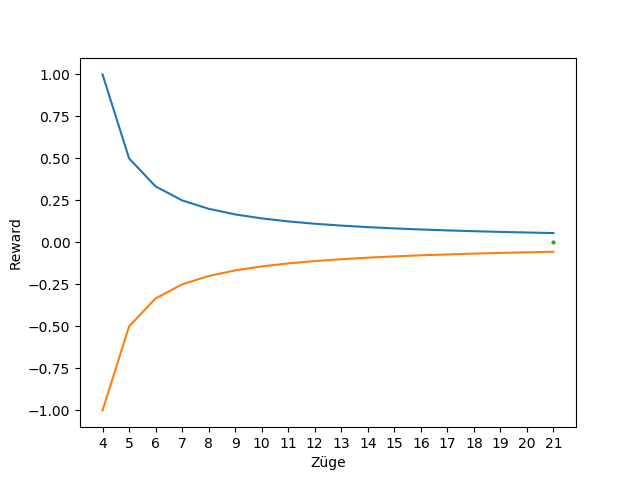
\includegraphics[scale=0.5]{reward_plot.png}
  \centering
  \caption{Reward Funktion}
  \label{fig:reward_function}
\end{figure}

\subsection{Policy}
Da in Vier Gewinnt nur am Ende eines Spiels ein Reward ausgegeben werden kann, wird hier ein Deep Q-Network genutzt um das credit assignment problem zu lösen. 
Dieses Deep Q-Network wird nach einer Epsilon-Greedy Policy trainiert.

\subsubsection{Deep Q-Network}
Das Deep Q-Network speichert zu jedem gespielten Zug den derzeitigen State, die ausgeführte Aktion, den erhaltenen Reward, der daraus folgende State und ob der neue State die Episode beendet hat in sein Memory. Aus diesem Memory wird dann, mit der Funktion $experience\_replay$, eine gewisse Menge an zufälligen Proben genommen. Es ist sehr sinnvoll hier eine zufällige Probe zu nehmen, da sonst durch die in Reihe betrachteten Züge ein ungewollter Bias entstehen kann, welcher die Konvergenz des Trainingalgorithmuses stark verlangsamen kann
\cite[Seite 469]{HandsOn2017}.
Für diese Proben werden dann die Q-Values vorhergesagt. Mit diesen Q-Values wird dann das Q-Network trainiert. 
Dieser Prozess wird so häufig wiederholt, dass hierdurch die Q-Values immer genauer  werden und dadurch ergibt sich dann eine ziehlführende Policy.


\subsubsection{Epsilon-Greedy}
Als Unterstützung des Deep Q-Network wurde sich für die Epsilon-Greedy Policy entschieden, da diese sehr gut für Deep Q-Networks funktioniert \colorbox{red!30}{Source}. Epsilon-Greedy beschreibt das Verhalten des Agenten welches entweder explorativ oder ausbeutend ist. Ist das Verhalten explorativ entscheidet sich der Agent für einen Zug, den er vorher noch nicht oder selten gemacht hat um diesen zu erlernen. Ist das Verhalten ausbeutend so wird der Zug genommen welcher derzeitig die höchste Gewinnchance bietet. Zum Anfang des Lernens macht es natürlich Sinn, dass der Agent ganz viel erkundet, da er noch kein Wissen über das Spiel besitzt. Hat der Agent dann einige Spiele hinter sich kann er auf die ausbeutende Strategie umschalten. Um dieses Verhalten des erstigen Erkundens und späteren Ausbeutens zu ermöglichen nutzt die Epsilon-Greedy Policy die Formel: $np.random.rand())<1-\epsilon$. Gibt diese Formel $True$ zurück so wird erkundet, gibt sie $False$ aus wird ausgebeutet. Der Wert von Epsilon ist am Anfang etwas mehr als Null und wird wärend der Lernphase langsam erhöht bis er etwas weniger als 1 erreicht hat. Somit ist das Ergebniss der Formel am Anfang meistens $True$ und später meistens $False$. Somit kann das DQN am Anfang viele Daten bekommen um hieraus eine Policy zu erarbeiten und dann diese später nach und nach verbessern, wenn durch die Ausbeutung dann nach dieser Policy vorgegangen wird.


\section{Lernen vom Gegner}
Um das Lernen des Agenten zu verbessern wurde sich dazu entschieden, dass der Agent auch die Züge seines Gegners zum Lernen nutzen kann. Dies ist für Vier Gewinnt angemessen, da es sich um ein Spiel mit perfekter Information handelt. Es sind also jedem Spieler zum Zeitpunkt einer Entscheidung alle Informationen über das Spiel ersichtlich. Da ein menschlicher Anfänger in diesem Spiel, bei einer Niederlage an den Spielzügen seines Gegners lernen kann, wurde dies auch als sinnvoll für den Agenten angesehen. Hierfür mussten einige Anpassungen vorgenommen werden. Da der reinforcement learning Agent immer der erste der beiden Spieler ist, der seinen Zug macht, fehlen dem Deep Q-Network Informationen über den Zug nach seinem Gegner. 
Um diese Informationen zu erhalten wird das gesammte Spiel einen halben Zug in der Vergangenheit betrachtet. Somit kann dann der alte Zug des Gegners als der eigene betrachtet werden und der eigene Zug als Antwort auf diesen. Damit der reinforcement learning Agent dies dann verarbeiten kann muss noch das ganze Spielfeld negiert werden. Es werden also die Steine beider Spieler getauscht damit es wieder wie eine ganz normale Zugabfolge aussieht. 

\section{Graphische Darstellung}
Um die Effektivität der verschiedenen Versionen zu vergleichen wird der Reward in einem Graphen geplottet. Dies wird mit dem Paket pyplot von matplotlib gemacht. Beispiele hierfür findet man im Kapitel \ref{cha:Eval}  Evaluierung. \\


\section{Visualsierung des Spiels}
\label{sec:visualisierung}
Da das Spielfeld im Code nur als zweidimensionales Array,welches mit 1, 0 und -1 gefüllt ist, existiert ist es für den Menschen nicht so einfach zu erkennen was gerade im Spiel passiert ist. Hierfür wurde mit Hilfe des Python Pakets colorama eine Visualisierung erschaffen. Diese wandelt alle Felder in den Unicode Character 'BLACK CIRCLE' (U+25CF) um wobei die 1 Gelb und die -1 Rot eingefärbt werden. Hierzu wird noch der Hintergrund Blau eingefärbt um dem Design des Spiels möglichst nah zu kommen. \\
Abbildung \ref{fig:spielfeld_konsole} ist ein durch diese Weise erstelltes Spielfeld für das Interne Array \ref{fig:array}\\
\begin{figure}[ht]
\centering
$\begin{bmatrix}                                
[ \, & 0  & 0 & 0 & 0 & 0 & 0 & 0& ]\, \\                                               
[ \, & 0  & 0 & 0 & 0 & 0 & 0 & 0& ]\, \\  
[ \, & 0  & 0 & 0 & 0 & 0 & -1 & 0& ]\, \\  
[ \, & 0  & 0 & 0 & 0 & 0 & -1 & 0& ]\, \\  
[ \, & 1  & 0 & 1 & -1 & 0 & -1 & 0& ]\, \\  
[ \, & 1  & 1 & -1 & 1 & 0 & -1 & 1& ]\,                                               
\end{bmatrix}$
\caption{Array-Representation}
 \label{fig:array}
\end{figure}


\begin{figure}[h!]
  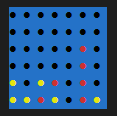
\includegraphics[width=117px,height=116px]{spielfeld_konsole.png}
  \centering
  \caption{Das Spielfeld auf der Konsole}
  \label{fig:spielfeld_konsole}
\end{figure}
